% Options for packages loaded elsewhere
\PassOptionsToPackage{unicode}{hyperref}
\PassOptionsToPackage{hyphens}{url}
%
\documentclass[
    ]{article}
    \usepackage[a4paper,top=2cm,bottom=1.5cm,left=2cm,right=2cm,marginparwidth=1.5cm]{geometry}
    \usepackage{graphicx}
    % \usepackage[french]{babel}
    \usepackage{fancyhdr}
    \usepackage{setspace}
    \usepackage[font=small, labelfont=bf]{caption}
    \usepackage[colorlinks=true, allcolors=blue]{hyperref}
    \usepackage{incgraph}
    \usepackage{algorithm}
    \usepackage{algorithmic}
    \usepackage[ruled,vlined]{algorithm2e}
    \usepackage{pdfpages}
\usepackage{lmodern}
\usepackage{amssymb,amsmath}
\usepackage{ifxetex,ifluatex}
\ifnum 0\ifxetex 1\fi\ifluatex 1\fi=0 % if pdftex
  \usepackage[T1]{fontenc}
  \usepackage[utf8]{inputenc}
  \usepackage{textcomp} % provide euro and other symbols
\else % if luatex or xetex
  \usepackage{unicode-math}
  \defaultfontfeatures{Scale=MatchLowercase}
  \defaultfontfeatures[\rmfamily]{Ligatures=TeX,Scale=1}
\fi
% Use upquote if available, for straight quotes in verbatim environments
\IfFileExists{upquote.sty}{\usepackage{upquote}}{}
\IfFileExists{microtype.sty}{% use microtype if available
  \usepackage[]{microtype}
  \UseMicrotypeSet[protrusion]{basicmath} % disable protrusion for tt fonts
}{}
\makeatletter
\@ifundefined{KOMAClassName}{% if non-KOMA class
  \IfFileExists{parskip.sty}{%
    \usepackage{parskip}
  }{% else
    \setlength{\parindent}{0pt}
    \setlength{\parskip}{6pt plus 2pt minus 1pt}}
}{% if KOMA class
  \KOMAoptions{parskip=half}}
\makeatother
\usepackage{xcolor}
\IfFileExists{xurl.sty}{\usepackage{xurl}}{} % add URL line breaks if available
\IfFileExists{bookmark.sty}{\usepackage{bookmark}}{\usepackage{hyperref}}
\hypersetup{
  hidelinks,
  pdfcreator={LaTeX via pandoc}}
\urlstyle{same} % disable monospaced font for URLs
\usepackage{color}
\usepackage{fancyvrb}
\newcommand{\VerbBar}{|}
\newcommand{\VERB}{\Verb[commandchars=\\\{\}]}
\DefineVerbatimEnvironment{Highlighting}{Verbatim}{commandchars=\\\{\}}
% Add ',fontsize=\small' for more characters per line
\newenvironment{Shaded}{}{}
\newcommand{\AlertTok}[1]{\textcolor[rgb]{1.00,0.00,0.00}{\textbf{#1}}}
\newcommand{\AnnotationTok}[1]{\textcolor[rgb]{0.38,0.63,0.69}{\textbf{\textit{#1}}}}
\newcommand{\AttributeTok}[1]{\textcolor[rgb]{0.49,0.56,0.16}{#1}}
\newcommand{\BaseNTok}[1]{\textcolor[rgb]{0.25,0.63,0.44}{#1}}
\newcommand{\BuiltInTok}[1]{#1}
\newcommand{\CharTok}[1]{\textcolor[rgb]{0.25,0.44,0.63}{#1}}
\newcommand{\CommentTok}[1]{\textcolor[rgb]{0.38,0.63,0.69}{\textit{#1}}}
\newcommand{\CommentVarTok}[1]{\textcolor[rgb]{0.38,0.63,0.69}{\textbf{\textit{#1}}}}
\newcommand{\ConstantTok}[1]{\textcolor[rgb]{0.53,0.00,0.00}{#1}}
\newcommand{\ControlFlowTok}[1]{\textcolor[rgb]{0.00,0.44,0.13}{\textbf{#1}}}
\newcommand{\DataTypeTok}[1]{\textcolor[rgb]{0.56,0.13,0.00}{#1}}
\newcommand{\DecValTok}[1]{\textcolor[rgb]{0.25,0.63,0.44}{#1}}
\newcommand{\DocumentationTok}[1]{\textcolor[rgb]{0.73,0.13,0.13}{\textit{#1}}}
\newcommand{\ErrorTok}[1]{\textcolor[rgb]{1.00,0.00,0.00}{\textbf{#1}}}
\newcommand{\ExtensionTok}[1]{#1}
\newcommand{\FloatTok}[1]{\textcolor[rgb]{0.25,0.63,0.44}{#1}}
\newcommand{\FunctionTok}[1]{\textcolor[rgb]{0.02,0.16,0.49}{#1}}
\newcommand{\ImportTok}[1]{#1}
\newcommand{\InformationTok}[1]{\textcolor[rgb]{0.38,0.63,0.69}{\textbf{\textit{#1}}}}
\newcommand{\KeywordTok}[1]{\textcolor[rgb]{0.00,0.44,0.13}{\textbf{#1}}}
\newcommand{\NormalTok}[1]{#1}
\newcommand{\OperatorTok}[1]{\textcolor[rgb]{0.40,0.40,0.40}{#1}}
\newcommand{\OtherTok}[1]{\textcolor[rgb]{0.00,0.44,0.13}{#1}}
\newcommand{\PreprocessorTok}[1]{\textcolor[rgb]{0.74,0.48,0.00}{#1}}
\newcommand{\RegionMarkerTok}[1]{#1}
\newcommand{\SpecialCharTok}[1]{\textcolor[rgb]{0.25,0.44,0.63}{#1}}
\newcommand{\SpecialStringTok}[1]{\textcolor[rgb]{0.73,0.40,0.53}{#1}}
\newcommand{\StringTok}[1]{\textcolor[rgb]{0.25,0.44,0.63}{#1}}
\newcommand{\VariableTok}[1]{\textcolor[rgb]{0.10,0.09,0.49}{#1}}
\newcommand{\VerbatimStringTok}[1]{\textcolor[rgb]{0.25,0.44,0.63}{#1}}
\newcommand{\WarningTok}[1]{\textcolor[rgb]{0.38,0.63,0.69}{\textbf{\textit{#1}}}}
\setlength{\emergencystretch}{3em} % prevent overfull lines
\providecommand{\tightlist}{%
  \setlength{\itemsep}{0pt}\setlength{\parskip}{0pt}}
\setcounter{secnumdepth}{-\maxdimen} % remove section numbering




\newcommand{\HRule}[1]{\rule{\linewidth}{#1}}
\onehalfspacing

\pagestyle{fancy}
\fancyhf{}
\setlength\headheight{15pt}
 \setlength{\marginparwidth}{2cm}
\usepackage[
    left = \flqq{},% 
    right = \frqq{},% 
    leftsub = \flq{},% 
    rightsub = \frq{} %
    ]{dirtytalk}
    \setlength\headheight{15pt}
    
    % Ligne de Haut de page (Nom + UV)
    \fancyhead[L]{SAVARY Tobias BUREAU Marius UTC - GI02} 
    \fancyhead[R]{SR02 - Rapport Threads}

    % Bas de page (Nomero de page + UTC)
    \fancyfoot[R]{\thepage}
    \fancyfoot[L]{Université de Technologie de Compiègne}
     \setlength {\marginparwidth}{2cm}
     \renewcommand{\footrulewidth}{.5pt}

\begin{document}

\title{ 
   \begin{center}
           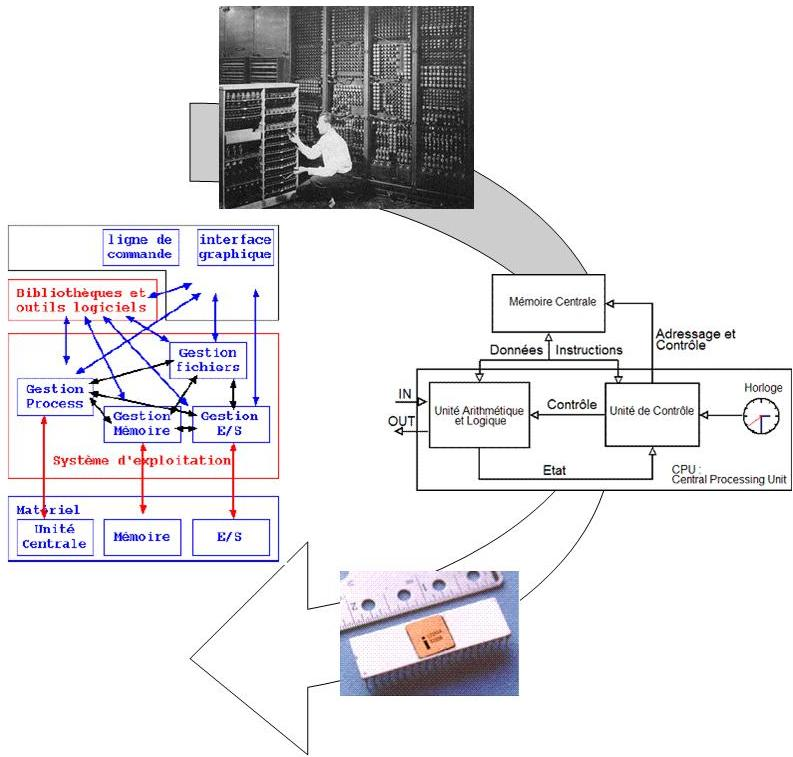
\includegraphics[width=5cm]{img/SR02.jpg} \hspace*{1cm}
           
\includegraphics[width=9cm]{img/logo_UTC.png} \\ [2cm]
   \end{center}
		\HRule{2pt} \\

    % Titre du Rapport
		\LARGE \textbf{Rapport TD8:\\Threads \\ Crible d’Eratosthenes} 
		\HRule{2pt} \\ [5.5cm]


		\normalsize  
    % Nom de l'auteur
        \author{
            Tobias SAVARY \\[0.5cm]
            Marius BUREAU \\[0.5cm]
           \\[1cm]
        }
		}
    % Année universitaire
		\maketitle
        \begin{center}
            Année universitaire 2022/2023
        \end{center}
\pagebreak

% Table des matières 
\tableofcontents

\pagebreak

% \hypertarget{sr02-td-8-threads-crible-deratosthenes}{%
% \section{SR02 : TD 8 (Threads : Crible
% d'Eratosthenes)}\label{sr02-td-8-threads-crible-deratosthenes}}

\hypertarget{tache-1}{%
\subsection{Tache 1}\label{tache-1}}

\hypertarget{duxe9rouler-lexuxe9cution-de-cette-algorithme-avec-n20}{%
\subsubsection{Dérouler l'exécution de cette algorithme avec
n=20}\label{duxe9rouler-lexuxe9cution-de-cette-algorithme-avec-n20}}

\begin{enumerate}
\def\labelenumi{\arabic{enumi}.}
\tightlist
\item
\end{enumerate}

\begin{enumerate}
\def\labelenumi{\Alph{enumi})}
\item
  Initialisation du tableau\\
  A = {[}Vrai, Vrai, Vrai, Vrai, Vrai, Vrai, Vrai, Vrai, Vrai, Vrai,
  Vrai, Vrai, Vrai, Vrai, Vrai, Vrai, Vrai, Vrai, Vrai{]}
\item
  Boucle for sur i\\
  Parcour des valeurs de i de 2 à \(\sqrt{20}\) , soit i = 2, 3, 4.
\end{enumerate}

i = 2:

\begin{verbatim}
A[2] est vrai,  
On met à faux toutes les valeurs de j = 4, 6, 8, 10, 12, 14, 16, 18, 20  
dans le tableau A.  
Le tableau A devient : [Vrai, Vrai, Faux, Vrai, Faux, Vrai, Faux,  
Vrai, Faux, Vrai, Faux, Vrai, Faux, Vrai, Faux, Vrai, Faux, Vrai, Faux]  
\end{verbatim}

i = 3:

\begin{verbatim}
A[3] est vrai,  
On met à faux toutes les valeurs de j = 9, 12, 15, 18 dans le tableau A.  
Le tableau A devient : [Vrai, Vrai, Faux, Vrai, Faux, Vrai, Faux, Faux,  
Faux, Vrai, Faux, Vrai, Faux, Faux, Faux, Vrai, Faux, Vrai, Faux]  
\end{verbatim}

i = 4:

\begin{verbatim}
A[4] est faux, on passe à l'itération suivante.  
\end{verbatim}

\begin{enumerate}
\def\labelenumi{\Alph{enumi})}
\setcounter{enumi}{2}
\tightlist
\item
  Résultat final\\
  Après avoir parcouru toutes les valeurs de i, le tableau A contient
  les informations sur les nombres premiers jusqu'à 20. Les indices pour
  lesquels A{[}i{]} est vrai correspondent aux nombres premiers.
\end{enumerate}

Le tableau A final est le suivant : {[}Vrai, Vrai, Faux, Vrai, Faux,
Vrai, Faux, Faux, Faux, Vrai, Faux, Vrai, Faux, Faux, Faux, Vrai, Faux,
Vrai, Faux{]}

Donc, les nombres premiers jusqu'à 20 sont : 2, 3, 5, 7, 11, 13, 17, 19.

\begin{enumerate}
\def\labelenumi{\arabic{enumi}.}
\setcounter{enumi}{1}
\tightlist
\item
  La boucle interne commence à \(i^2\) au lieu de 0 ou i pour des
  raisons d'efficacité.
\end{enumerate}

L'algorithme utilise le crible d'Ératosthène pour trouver les nombres
premiers jusqu'à n.~L'idée du crible d'Ératosthène est que tous les
multiples d'un nombre ne sont pas premiers, ils peuvent donc être
supprimés. Ainsi, au lieu de parcourir tous les multiples de i, la
boucle interne commence à \(i^2\) pour éliminer tous les multiples
précédents qui ont déjà été marqués comme non premiers par des valeurs
de i plus petites.

Supposons que i soit un nombre premier. Si nous commençons à i ou à une
valeur inférieure à \(i^2\), on passe sur des multiples de nombres
premiers précédents, ce qui serait redondant. Par exemple, si i = 3, en
commencant à \(3^2\) = 9 on ne passe pas par 6 (multiple de 2) et 3
(multiple de 3), car ils ont déjà été testés précédemment.

En commençant à \(i^2\), on est sur que chaque multiple antérieur a déjà
été marqué comme non premier, ce qui permet de réduire le nombre
d'itérations. Ce départ à \(i^2\) constitue donc principalement une
optimisation de l'algorithme puisque les itérations avant \(i^2\) ne
seraient pas nécéssaires.

\begin{enumerate}
\def\labelenumi{\arabic{enumi}.}
\setcounter{enumi}{2}
\tightlist
\item
  La première boucle s'exécute jusqu'à \(\sqrt{n}\) pour des raisons
  d'efficacité. L'objectif de cette boucle est de marquer tous les
  multiples des nombres premiers jusqu'à \(\sqrt{n}\) comme non
  premiers.
\end{enumerate}

Si \(\sqrt{n}\) n'est pas un entier, nous prenons la partie entière
inférieur de \(\sqrt{n}\).

Dans le cas où \(\sqrt{n}\) est un entier, la première boucle s'exécute
normalement de 2 à \(\sqrt{n}\) inclus, couvrant ainsi tous les
multiples des nombres premiers jusqu'à \(\sqrt{n}\).

L'objectif est de limiter le nombre d'itérations nécessaires, car après
\(\sqrt{n}\), nous n'avons plus besoin de vérifier les multiples des
nombres premiers plus grands que \(\sqrt{n}\), car ils ont déjà été
traités lors des itérations précédentes.(Cette propriété est une
propriété toujours vrai pour les nombres premiers.)

Lorsque nous cherchons tous les nombres premiers inférieurs ou égale à
N, nous pouvons effectivement itérer sur les entiers i de 2 à N.

Cependant, il n'est pas nécessaire de vérifier tous les nombres jusqu'à
N. Il suffit de vérifier jusqu'à la racine carrée de N. Cela est dû au
fait que si un nombre non premier a un facteur qui est plus grand que sa
racine carrée, il aurait déjà été multiplié par un autre facteur plus
petit qui est inférieur à sa racine carrée.

Par conséquent, en vérifiant seulement jusqu'à la racine carrée de N,
nous couvrons tous les cas et nous évitons les tests redondants.

``D'après le théorème des diviseurs premiers, si n n'est divisible par
aucun des nombres premiers inférieur ou égaux à sa racine carrée, on
peut affirmer qu'il est premier.''

Cela permet d'optimiser l'algorithme et d'améliorer son efficacité.

\pagebreak

\hypertarget{tache-2}{%
\subsection{Tache 2}\label{tache-2}}
Explication de l'algorithme avec les commentaires

\begin{Shaded}
\begin{Highlighting}[]
\PreprocessorTok{\#include }\ImportTok{\textless{}stdio.h\textgreater{}}
\PreprocessorTok{\#include }\ImportTok{\textless{}stdlib.h\textgreater{}}
\PreprocessorTok{\#include }\ImportTok{\textless{}math.h\textgreater{}}
\PreprocessorTok{\#include }\ImportTok{\textless{}time.h\textgreater{}}

\CommentTok{//Fonction qui permet de calculer les nombres premiers de 2 à n}
\DataTypeTok{void}\NormalTok{ Eratosthenes(}\DataTypeTok{unsigned} \DataTypeTok{long}\NormalTok{ n, }\DataTypeTok{unsigned} \DataTypeTok{long}\NormalTok{ *tab) \{}
\CommentTok{// Initialisation du tableau de booleen à vrai}
    \ControlFlowTok{for}\NormalTok{ (}\DataTypeTok{unsigned} \DataTypeTok{long}\NormalTok{ i = }\DecValTok{2}\NormalTok{; i \textless{}= n; i++) \{}
\NormalTok{        tab[i] = }\DecValTok{1}\NormalTok{;}
\NormalTok{    \}}
\CommentTok{    // Calcul de l'interval de test ( 1 jusqu'à racine de n)}
    \DataTypeTok{unsigned} \DataTypeTok{long}\NormalTok{ racine = $\textbackslash{}sqrt\{n\}$;}
    \CommentTok{   //Boucle de test pour voir si ce sont des nombres premiers ou non}
    \ControlFlowTok{for}\NormalTok{ (}\DataTypeTok{unsigned} \DataTypeTok{long}\NormalTok{ i = }\DecValTok{2}\NormalTok{; i \textless{}= racine; i++) \{}
        \CommentTok{// Si le nombre est premier}
        \ControlFlowTok{if}\NormalTok{ (tab[i] == }\DecValTok{1}\NormalTok{) \{}
            \CommentTok{ // On enlève tous les multiples de i}
            \ControlFlowTok{for}\NormalTok{ (}\DataTypeTok{unsigned} \DataTypeTok{long}\NormalTok{ j = i * i; j \textless{}= n; j += i) \{}
\NormalTok{                tab[j] = }\DecValTok{0}\NormalTok{;}
\NormalTok{            \}}
\NormalTok{    \}\}\}}
\CommentTok{//Fonction l'affichage du tableau}
\DataTypeTok{void}\NormalTok{ PrintTab(}\DataTypeTok{unsigned} \DataTypeTok{long}\NormalTok{ n, }\DataTypeTok{unsigned} \DataTypeTok{long}\NormalTok{ *tab) \{}
    \ControlFlowTok{for}\NormalTok{ (}\DataTypeTok{unsigned} \DataTypeTok{long}\NormalTok{ i = }\DecValTok{2}\NormalTok{; i \textless{}= n; i++) \{}
        \ControlFlowTok{if}\NormalTok{ (tab[i] == }\DecValTok{1}\NormalTok{) \{}
\NormalTok{            printf(}\StringTok{"\%lu "}\NormalTok{, i);}
\NormalTok{        \}}
\NormalTok{    \}}
\NormalTok{    printf(}\StringTok{"}\SpecialCharTok{\textbackslash{}n}\StringTok{"}\NormalTok{);}
\NormalTok{\}}
\DataTypeTok{int}\NormalTok{ main(}\DataTypeTok{int}\NormalTok{ argc, }\DataTypeTok{char}\NormalTok{ **argv) \{}
    \CommentTok{   // On vérifie que seulement 1 argument est passé au programme}
    \ControlFlowTok{if}\NormalTok{(argc != }\DecValTok{2}\NormalTok{) \{}
\NormalTok{        printf(}\StringTok{"Usage: \%s \textless{}n\textgreater{}}\SpecialCharTok{\textbackslash{}n}\StringTok{"}\NormalTok{, argv[}\DecValTok{0}\NormalTok{]);}
        \ControlFlowTok{return} \DecValTok{1}\NormalTok{;}
\NormalTok{    \}}
    \CommentTok{    // Conversion de l'argument en long}
    \DataTypeTok{unsigned} \DataTypeTok{long}\NormalTok{ n = atol(argv[}\DecValTok{1}\NormalTok{]);}
    \CommentTok{   // Aucun n appartenant à [0;1] n'est premier, on traite donc uniquement les cas ou n > 1}
    \ControlFlowTok{if}\NormalTok{ (n \textgreater{} }\DecValTok{1}\NormalTok{) \{}
        \CommentTok{ // Création du tableau de booleen : n+1 car l'index correspond }
        \CommentTok{ //à un nombre et la valeure de l'index le booleen (1 = premier, 0 = pas premier)}
        \CommentTok{ //0 étant en nombre et les indices commencant à 0, }
        \CommentTok{ //nécessiter de rajouter une case au tableau}
    \DataTypeTok{unsigned} \DataTypeTok{long}\NormalTok{ *tab = (}\DataTypeTok{unsigned} \DataTypeTok{long}\NormalTok{ *)malloc((n+}\DecValTok{1}\NormalTok{) * }\KeywordTok{sizeof}\NormalTok{(}\DataTypeTok{unsigned} \DataTypeTok{long}\NormalTok{));}
    \CommentTok{        // Variables pour récupérer le temps}
\NormalTok{        clock\_t start, end;}
        \DataTypeTok{double}\NormalTok{ temps\_execution;}
        \CommentTok{// On lance le chronomètre}
\NormalTok{        start = clock();}
\NormalTok{        Eratosthenes(n, tab);}
\NormalTok{        end = clock();}
\NormalTok{        temps\_execution = ((}\DataTypeTok{double}\NormalTok{) (end {-} start)) / CLOCKS\_PER\_SEC;}
\NormalTok{        printf(}\StringTok{"\%f}\SpecialCharTok{\textbackslash{}n}\StringTok{"}\NormalTok{, temps\_execution);}
        \CommentTok{// PrintTab(100, tab);}
        \CommentTok{// Libération du tableau}
\NormalTok{        free(tab);}
\NormalTok{    \} }\ControlFlowTok{else}\NormalTok{ \{}
\NormalTok{        printf(}\StringTok{"n doit être supérieur à 1.}\SpecialCharTok{\textbackslash{}n}\StringTok{"}\NormalTok{);}
\NormalTok{    \}}
    \ControlFlowTok{return} \DecValTok{0}\NormalTok{;}
\NormalTok{\}}
\end{Highlighting}
\end{Shaded}
\pagebreak

\hypertarget{tache-3}{%
\subsection{Tache 3}\label{tache-3}}
\begin{Shaded}
\begin{Highlighting}[]
\PreprocessorTok{\#include }\ImportTok{\textless{}stdio.h\textgreater{}}
\PreprocessorTok{\#include }\ImportTok{\textless{}stdlib.h\textgreater{}}
\PreprocessorTok{\#include }\ImportTok{\textless{}math.h\textgreater{}}
\PreprocessorTok{\#include }\ImportTok{\textless{}pthread.h\textgreater{}}
\CommentTok{// Constante }
\PreprocessorTok{\#define k 7}

\CommentTok{// Strucutre qui va permettre d'envoyer plusieurs variables à un thread}
\KeywordTok{typedef} \KeywordTok{struct}
\NormalTok{\{}
    \DataTypeTok{unsigned} \DataTypeTok{long}\NormalTok{ *tab;}
    \DataTypeTok{unsigned} \DataTypeTok{long}\NormalTok{ i;}
    \DataTypeTok{unsigned} \DataTypeTok{long}\NormalTok{ n;}
    \DataTypeTok{unsigned} \DataTypeTok{long}\NormalTok{ racine;}
\NormalTok{    pthread\_mutex\_t *mutex;}
\NormalTok{\} ArgumentThread;}

\CommentTok{//Fonction utiliser par les thread}
\DataTypeTok{void}\NormalTok{ *fonctionThread(}\DataTypeTok{void}\NormalTok{ *argument)}
\NormalTok{\{}
\CommentTok{    // Initialisation des variables}
\NormalTok{    ArgumentThread *arg = (ArgumentThread *)argument;}
    \CommentTok{    // Tableau de booleen}
    \DataTypeTok{unsigned} \DataTypeTok{long}\NormalTok{ *tab = arg{-}\textgreater{}tab;}
    \CommentTok{    // Valeur de i à tester}
    \DataTypeTok{unsigned} \DataTypeTok{long}\NormalTok{ i = arg{-}\textgreater{}i;}
    \DataTypeTok{unsigned} \DataTypeTok{long}\NormalTok{ n = arg{-}\textgreater{}n;}
    \CommentTok{ \\  Ici le choix de l'implémentation des thread à été définis a ce que les threads }
    \CommentTok{ \\ commencent à une valeure donnée (i) et se termine à racine(n) avec un pas de k }
    \CommentTok{ \\ Ce choix d'implémentation a été réfléchi : étant donné que plus i est bas, }
    \CommentTok{ \\ plus il y a de multiple à enlever, autant traiter les nombres les plus petits en premier }
    \CommentTok{ \\ On répartit donc les petits nombres à chaque thread puis on incrémente i du nombre de thread   }
    \ControlFlowTok{for}\NormalTok{ (}\DataTypeTok{unsigned} \DataTypeTok{long}\NormalTok{ t = i; t \textless{}= arg{-}\textgreater{}racine; t += k)}
\NormalTok{    \{}
        \ControlFlowTok{if}\NormalTok{ (tab[t] == }\DecValTok{1}\NormalTok{)}
\NormalTok{        \{}
\CommentTok{            // On utilise un mutex pour éviter l'accés concurentiel}
\NormalTok{            pthread\_mutex\_lock(arg{-}\textgreater{}mutex);}
            \ControlFlowTok{for}\NormalTok{ (}\DataTypeTok{unsigned} \DataTypeTok{long}\NormalTok{ j = t * t; j \textless{}= n; j += t)}
\NormalTok{            \{}
\NormalTok{                tab[j] = }\DecValTok{0}\NormalTok{;}
\NormalTok{            \}}
\CommentTok{      //Libération du mutex}
\NormalTok{            pthread\_mutex\_unlock(arg{-}\textgreater{}mutex);}
\NormalTok{        \}}
\NormalTok{    \}}
\CommentTok{       // Retour du thread}
\NormalTok{    pthread\_exit(NULL);}
\NormalTok{\}}
\end{Highlighting}
\end{Shaded}
\begin{Shaded}
    \begin{Highlighting}[]
\DataTypeTok{void}\NormalTok{ Eratosthenes(}\DataTypeTok{unsigned} \DataTypeTok{long}\NormalTok{ n, }\DataTypeTok{unsigned} \DataTypeTok{long}\NormalTok{ *tab)}
\NormalTok{\{}
\CommentTok{    // Initialisation du tableau de thread}
\NormalTok{    pthread\_t *thread = malloc(}\KeywordTok{sizeof}\NormalTok{(pthread\_t) * k);}
    \DataTypeTok{unsigned} \DataTypeTok{long}\NormalTok{ indexThread = }\DecValTok{0}\NormalTok{;}
    \CommentTok{// Creation du mutex}
\NormalTok{    pthread\_mutex\_t mutex;}
\NormalTok{    pthread\_mutex\_init(\&mutex, NULL);}

\CommentTok{    // Initialisation des thread }
    \ControlFlowTok{for}\NormalTok{ (}\DataTypeTok{int}\NormalTok{ cpt = }\DecValTok{0}\NormalTok{; cpt \textless{} k; cpt++)}
\NormalTok{    \{}
\CommentTok{    	// Data a envoyer au thread}
\NormalTok{        ArgumentThread *arg = malloc(}\KeywordTok{sizeof}\NormalTok{(ArgumentThread));}
\NormalTok{        arg{-}\textgreater{}tab = tab;}
\CommentTok{// Ici i = 2 + cpt car come dit précédemment on veut traiter les petits nombre en premier }
\NormalTok{        arg{-}\textgreater{}i = }\DecValTok{2}\NormalTok{ + cpt;}
\NormalTok{        arg{-}\textgreater{}n = n;}
\NormalTok{        arg{-}\textgreater{}racine = $\textbackslash{}sqrt\{n\}$;}
\NormalTok{        arg{-}\textgreater{}mutex = \&mutex;}
        
\CommentTok{        // Création des threads}
\NormalTok{        pthread\_create(\&thread[indexThread], NULL, fonctionThread, arg);}
\NormalTok{        indexThread++;}
\NormalTok{    \}}
\CommentTok{    // On attends la fin de tous les threads}
    \ControlFlowTok{for}\NormalTok{ (}\DataTypeTok{unsigned} \DataTypeTok{long}\NormalTok{ i = }\DecValTok{0}\NormalTok{; i \textless{} indexThread; i++)}
\NormalTok{    \{}
\NormalTok{        pthread\_join(thread[i], NULL);}
\NormalTok{    \}}
\CommentTok{    // Libération du tableau de thread et du mutex}
\NormalTok{    free(thread);}
\NormalTok{    pthread\_mutex\_destroy(\&mutex);}
\NormalTok{\}}

\DataTypeTok{void}\NormalTok{ PrintTab(}\DataTypeTok{unsigned} \DataTypeTok{long}\NormalTok{ n, }\DataTypeTok{unsigned} \DataTypeTok{long}\NormalTok{ *tab)}
\NormalTok{\{}
    \CommentTok{// Affichage des nombres premiers}
    \ControlFlowTok{for}\NormalTok{ (}\DataTypeTok{unsigned} \DataTypeTok{long}\NormalTok{ i = }\DecValTok{2}\NormalTok{; i \textless{}= n; i++)}
\NormalTok{    \{}
\NormalTok{        printf(}\StringTok{"\%ld "}\NormalTok{, tab[i]);}
\NormalTok{    \}}
\NormalTok{    printf(}\StringTok{"}\SpecialCharTok{\textbackslash{}n}\StringTok{"}\NormalTok{);}
\NormalTok{\}}

\DataTypeTok{void}\NormalTok{ PrintIndex(}\DataTypeTok{unsigned} \DataTypeTok{long}\NormalTok{ n, }\DataTypeTok{unsigned} \DataTypeTok{long}\NormalTok{ *tab)}
\NormalTok{\{}
    \DataTypeTok{int}\NormalTok{ cpt = }\DecValTok{0}\NormalTok{;}
    \CommentTok{// Affichage des nombres premiers}
    \ControlFlowTok{for}\NormalTok{ (}\DataTypeTok{unsigned} \DataTypeTok{long}\NormalTok{ i = }\DecValTok{2}\NormalTok{; i \textless{}= n; i++)}
\NormalTok{    \{}
        \ControlFlowTok{if}\NormalTok{ (tab[i] == }\DecValTok{1}\NormalTok{)}
\NormalTok{        \{}
\NormalTok{            cpt++;}
            \CommentTok{// printf("\%ld ", i);}
\NormalTok{        \}}
\NormalTok{    \}}
    \CommentTok{// printf("\%d\textbackslash{}n", cpt);}
    \CommentTok{// printf("\textbackslash{}n");}
\NormalTok{\}}

\DataTypeTok{int}\NormalTok{ main(}\DataTypeTok{int}\NormalTok{ argc, }\DataTypeTok{char}\NormalTok{ *argv[])}
\NormalTok{\{}
    \ControlFlowTok{if}\NormalTok{ (argc != }\DecValTok{2}\NormalTok{)}
\NormalTok{    \{}
\NormalTok{        printf(}\StringTok{"Usage: \%s n}\SpecialCharTok{\textbackslash{}n}\StringTok{"}\NormalTok{, argv[}\DecValTok{0}\NormalTok{]);}
        \ControlFlowTok{return} \DecValTok{0}\NormalTok{;}
\NormalTok{    \}}
    \DataTypeTok{unsigned} \DataTypeTok{long}\NormalTok{ n = atol(argv[}\DecValTok{1}\NormalTok{]);}

    \ControlFlowTok{if}\NormalTok{ (n \textgreater{} }\DecValTok{1}\NormalTok{)}
\NormalTok{    \{}
\CommentTok{   // Création du tableau de booleen : n+1 car l'index correspond }
\CommentTok{// à un nombre et la valeure de l'index le booleen (1 = premier, 0 = pas premier) }
\CommentTok{//0 étant en nombre et les indices commencant à 0, nécessiter de rajouter une case au tableau }
        \DataTypeTok{unsigned} \DataTypeTok{long}\NormalTok{ *tab = (}\DataTypeTok{unsigned} \DataTypeTok{long}\NormalTok{ *)malloc((n + }\DecValTok{1}\NormalTok{) * }\KeywordTok{sizeof}\NormalTok{(}\DataTypeTok{unsigned} \DataTypeTok{long}\NormalTok{));}
\NormalTok{        clock\_t start, end;}
        \DataTypeTok{double}\NormalTok{ temps\_execution;}
        \CommentTok{// Initialisation du tableau}
        \ControlFlowTok{for}\NormalTok{ (}\DataTypeTok{unsigned} \DataTypeTok{long}\NormalTok{ i = }\DecValTok{2}\NormalTok{; i \textless{}= n; i++)}
\NormalTok{        \{}
\NormalTok{            tab[i] = }\DecValTok{1}\NormalTok{;}
\NormalTok{        \}}
\CommentTok{         // Initialisation du chrono}
\NormalTok{        start = clock();}
\NormalTok{        Eratosthenes(n, tab);}
\CommentTok{        // Fin du chrono}
\NormalTok{        end = clock();}
\CommentTok{         // Calcul du temps}
\NormalTok{        temps\_execution = ((}\DataTypeTok{double}\NormalTok{)(end {-} start)) / CLOCKS\_PER\_SEC;}
\NormalTok{        printf(}\StringTok{"\%f}\SpecialCharTok{\textbackslash{}n}\StringTok{"}\NormalTok{, temps\_execution);}

\NormalTok{        PrintIndex(n, tab);}
        \CommentTok{// PrintTab(n, tab);}
        \CommentTok{// Libération du tableau}
\NormalTok{        free(tab);}
\NormalTok{    \}}
    \ControlFlowTok{else}
\NormalTok{    \{}
\NormalTok{        printf(}\StringTok{"n doit être supérieur à 1.}\SpecialCharTok{\textbackslash{}n}\StringTok{"}\NormalTok{);}
\NormalTok{    \}}

    \ControlFlowTok{return} \DecValTok{0}\NormalTok{;}
\NormalTok{\}}
\end{Highlighting}
\end{Shaded}
\pagebreak

/!~GRAPH 1\\
\pagebreak 

\hypertarget{tache-4-interpruxe9tation-des-ruxe9sultats}{%
\subsection{Tache 4: Interprétation des
résultats}\label{tache-4-interpruxe9tation-des-ruxe9sultats}}

Pour chaque test, que ce soit dans la tâche 4 ou la tâche 5, nous avons
pris la moyenne des temps d'exécutions pour 30 tests afin de réaliser
les graphiques. Vous trouverez ces valeurs dans le fichier EXCEL.

La similarité des points pour 500 000 et 1 000 000 indique que les temps
d'exécution sont assez uniformes, ce qui suggère que les différentes
implémentations ne génèrent pas de performances nettement meilleures.

À partir de la valeur 2 000 000, une dispersion des valeurs devient
apparente, ce qui met en évidence les différences d'implémentation de
manière plus marquée. On peut observer deux groupes principaux de
valeurs. Le premier groupe se situe autour de 0,030 secondes, tandis que
le second groupe se situe autour de 0,036 secondes.

Le premier groupe est constitué des implémentations utilisant des
threads pour les valeurs de k égales à 1, 2, 3, 4 et 6. Le second groupe
comprend l'implémentation séquentielle ainsi que celle utilisant des
threads pour les valeurs de k égales à 5 et 7.

En utilisant la valeur 4 000 000, ces résultats précédents sont
confirmés, et la valeur optimale de k (k=3) est obtenue. On observe que
pour les valeurs de k égales à 1, 2, 4 et 6, les temps d'exécution
restent assez proches. Ainsi, les différences de nombre de threads n'ont
pas d'impact significatif sur le temps d'exécution des programmes.\\
Malgrè l'augmentation du nombre de thread, on remarque que les temps
d'exécutions sont plus longs que lorsqu'on utilise moins de thread. Cela
est dû à la gestion des threads, et notamment à leurs créations, qui
demmandent du temps et des ressources. Il y a donc un équilibre à
trouver lorsque l'on veut utiliser des threads.

\hypertarget{intervalle-de-confiance}{%
\subsubsection{Intervalle de confiance}\label{intervalle-de-confiance}}

Afin de calculer l'intervalle de confiance sur ces valeurs, nous pouvons
poser \(X\) la variable aléatoire repésentant le temps d'exécution du
programme. Ensuite, nous devons calculer la moyenne de x
(\(\overline{x}\)) ainsi que son équart type (\(\sigma\)).\\
Nous pouvons poser un niveau de confiance \(\alpha^{*}\).\\
Dans notre cas, on peut prendre un niveau de confiance
\(\alpha^{*} = 95\)\%. Si \[X \sim \mathcal{N}(\mu,\,\sigma^{2})\] On
pose :\\
Le quantile d'une loi de normale centrée réduite d'ordre \(\alpha^{*}\)
: \(u_{\alpha^{*}}\).\\
Le nombre de valeurs : \(n\).\\
L'intervalle de confiance est donné par la formule :\\
\begin{equation}
IC = [\overline{x} - u_{1- \frac{\alpha^{*}}{2}} \frac{\sigma}{\sqrt{n}} , \overline{x} + u_{1- \frac{\alpha^{*}}{2}} \frac{\sigma}{\sqrt{n}} ]
\end{equation}

Si la valeur observée se trouve dans l'intervalle de confiance, elle est
considérée comme correct, sinon, on considère qu'il y a une erreur.

\pagebreak

\hypertarget{tache-5}{%
\subsection{Tache 5}\label{tache-5}}

\hypertarget{accuxe9luxe9ration-de-la-boucle-interne}{%
\subsubsection{Accélération de la boucle
interne}\label{accuxe9luxe9ration-de-la-boucle-interne}}

Les deux cas distincts à traiter sont les suivants :

Cas spécial pour le nombre 2 : Le nombre 2 est le seul nombre premier
pair. Comme tous les autres nombres pairs sont exclus d'être premiers,
nous devons traiter le cas spécial du nombre 2 séparément. Par
conséquent, nous devons effectuer la boucle interne avec un pas de 2 au
lieu de i lorsque i est égal à 2.

Boucle interne pour les nombres impairs : Tous les autres nombres
premiers sont impairs. Par conséquent, nous pouvons ignorer les nombres
pairs lors de la boucle interne pour améliorer l'efficacité de
l'algorithme. Nous effectuons donc la boucle interne avec un pas de 2i
pour tous les nombres premiers impairs, en commençant par \(i^2\).

En résumé, le premier cas distinct est celui du nombre 2 où nous
utilisons un pas de 2 dans la boucle interne, tandis que le deuxième cas
distinct est celui des autres nombres premiers impairs, pour lesquels
nous utilisons également un pas de 2i dans la boucle interne.

\begin{Shaded}
\begin{Highlighting}[]
\PreprocessorTok{\#include }\ImportTok{\textless{}stdio.h\textgreater{}}
\PreprocessorTok{\#include }\ImportTok{\textless{}stdlib.h\textgreater{}}
\PreprocessorTok{\#include }\ImportTok{\textless{}math.h\textgreater{}}
\PreprocessorTok{\#include }\ImportTok{\textless{}pthread.h\textgreater{}}
\PreprocessorTok{\#define k 7}

\KeywordTok{typedef} \KeywordTok{struct}
\NormalTok{\{}
    \DataTypeTok{unsigned} \DataTypeTok{long}\NormalTok{ *tab;}
    \DataTypeTok{unsigned} \DataTypeTok{long}\NormalTok{ i;}
    \DataTypeTok{unsigned} \DataTypeTok{long}\NormalTok{ n;}
    \DataTypeTok{unsigned} \DataTypeTok{long}\NormalTok{ racine;}
\NormalTok{    pthread\_mutex\_t *mutex;}
\NormalTok{\} ArgumentThread;}

\DataTypeTok{void}\NormalTok{ *fonctionThread(}\DataTypeTok{void}\NormalTok{ *argument)}
\NormalTok{\{}
\NormalTok{    ArgumentThread *arg = (ArgumentThread *)argument;}
    \DataTypeTok{unsigned} \DataTypeTok{long}\NormalTok{ *tab = arg{-}\textgreater{}tab;}
    \DataTypeTok{unsigned} \DataTypeTok{long}\NormalTok{ i = arg{-}\textgreater{}i;}
    \DataTypeTok{unsigned} \DataTypeTok{long}\NormalTok{ n = arg{-}\textgreater{}n;}
    \ControlFlowTok{for}\NormalTok{ (}\DataTypeTok{unsigned} \DataTypeTok{long}\NormalTok{ t = i; t \textless{}= arg{-}\textgreater{}racine; t += k)}
\NormalTok{    \{}
        \ControlFlowTok{if}\NormalTok{ (tab[t] == }\DecValTok{1}\NormalTok{)}
\NormalTok{        \{}
\NormalTok{            pthread\_mutex\_lock(arg{-}\textgreater{}mutex);}
            \ControlFlowTok{if}\NormalTok{(t == }\DecValTok{2}\NormalTok{)}
\NormalTok{            \{}
                \ControlFlowTok{for}\NormalTok{ (}\DataTypeTok{unsigned} \DataTypeTok{long}\NormalTok{ j = t * t; j \textless{}= n; j += t)}
\NormalTok{                \{}
\NormalTok{                    tab[j] = }\DecValTok{0}\NormalTok{;}
\NormalTok{                \}}
\NormalTok{            \}}
            \ControlFlowTok{else}
\NormalTok{            \{}
                \ControlFlowTok{for}\NormalTok{ (}\DataTypeTok{unsigned} \DataTypeTok{long}\NormalTok{ j = t * t; j \textless{}= n; j += }\DecValTok{2}\NormalTok{*t)}
\NormalTok{                \{}
\NormalTok{                    tab[j] = }\DecValTok{0}\NormalTok{;}
\NormalTok{                \}}
\NormalTok{            \}}
\NormalTok{            pthread\_mutex\_unlock(arg{-}\textgreater{}mutex);}
\NormalTok{        \}}
\NormalTok{    \}}
\NormalTok{    pthread\_exit(NULL);}
\NormalTok{\}}

\DataTypeTok{void}\NormalTok{ Eratosthenes(}\DataTypeTok{unsigned} \DataTypeTok{long}\NormalTok{ n, }\DataTypeTok{unsigned} \DataTypeTok{long}\NormalTok{ *tab)}
\NormalTok{\{}
\NormalTok{    pthread\_t *thread = malloc(}\KeywordTok{sizeof}\NormalTok{(pthread\_t) * k);}
    \DataTypeTok{unsigned} \DataTypeTok{long}\NormalTok{ indexThread = }\DecValTok{0}\NormalTok{;}
\NormalTok{    pthread\_mutex\_t mutex;}
\NormalTok{    pthread\_mutex\_init(\&mutex, NULL);}
    
    \ControlFlowTok{for}\NormalTok{ (}\DataTypeTok{int}\NormalTok{ cpt = }\DecValTok{0}\NormalTok{; cpt \textless{} k; cpt++)}
\NormalTok{    \{}
\NormalTok{        ArgumentThread *arg = malloc(}\KeywordTok{sizeof}\NormalTok{(ArgumentThread));}
\NormalTok{        arg{-}\textgreater{}tab = tab;}
\NormalTok{        arg{-}\textgreater{}i = }\DecValTok{2}\NormalTok{ + cpt;}
\NormalTok{        arg{-}\textgreater{}n = n;}
\NormalTok{        arg{-}\textgreater{}racine = $\textbackslash{}sqrt\{n\}$;}
\NormalTok{        arg{-}\textgreater{}mutex = \&mutex;}
        
\NormalTok{        pthread\_create(\&thread[indexThread], NULL, fonctionThread, arg);}
\NormalTok{        indexThread++;}
\NormalTok{    \}}
    \ControlFlowTok{for}\NormalTok{ (}\DataTypeTok{unsigned} \DataTypeTok{long}\NormalTok{ i = }\DecValTok{0}\NormalTok{; i \textless{} indexThread; i++)}
\NormalTok{    \{}
\NormalTok{        pthread\_join(thread[i], NULL);}
\NormalTok{    \}}
\NormalTok{    free(thread);}
\NormalTok{    pthread\_mutex\_destroy(\&mutex);}
\NormalTok{\}}

\DataTypeTok{void}\NormalTok{ PrintTab(}\DataTypeTok{unsigned} \DataTypeTok{long}\NormalTok{ n, }\DataTypeTok{unsigned} \DataTypeTok{long}\NormalTok{ *tab)}
\NormalTok{\{}
    \CommentTok{// Affichage des nombres premiers}
    \ControlFlowTok{for}\NormalTok{ (}\DataTypeTok{unsigned} \DataTypeTok{long}\NormalTok{ i = }\DecValTok{2}\NormalTok{; i \textless{}= n; i++)}
\NormalTok{    \{}
\NormalTok{        printf(}\StringTok{"\%ld "}\NormalTok{, tab[i]);}
\NormalTok{    \}}
\NormalTok{    printf(}\StringTok{"}\SpecialCharTok{\textbackslash{}n}\StringTok{"}\NormalTok{);}
\NormalTok{\}}

\DataTypeTok{void}\NormalTok{ PrintIndex(}\DataTypeTok{unsigned} \DataTypeTok{long}\NormalTok{ n, }\DataTypeTok{unsigned} \DataTypeTok{long}\NormalTok{ *tab)}
\NormalTok{\{}
    \DataTypeTok{int}\NormalTok{ cpt = }\DecValTok{0}\NormalTok{;}
    \CommentTok{// Affichage des nombres premiers}
    \ControlFlowTok{for}\NormalTok{ (}\DataTypeTok{unsigned} \DataTypeTok{long}\NormalTok{ i = }\DecValTok{2}\NormalTok{; i \textless{}= n; i++)}
\NormalTok{    \{}
        \ControlFlowTok{if}\NormalTok{ (tab[i] == }\DecValTok{1}\NormalTok{)}
\NormalTok{        \{}
\NormalTok{            cpt++;}
            \CommentTok{// printf("\%ld ", i);}
\NormalTok{        \}}
\NormalTok{    \}}
    \CommentTok{// printf("\%d\textbackslash{}n", cpt);}
    \CommentTok{// printf("\textbackslash{}n");}
\NormalTok{\}}

\DataTypeTok{int}\NormalTok{ main(}\DataTypeTok{int}\NormalTok{ argc, }\DataTypeTok{char}\NormalTok{ *argv[])}
\NormalTok{\{}
    \ControlFlowTok{if}\NormalTok{ (argc != }\DecValTok{2}\NormalTok{)}
\NormalTok{    \{}
\NormalTok{        printf(}\StringTok{"Usage: \%s n}\SpecialCharTok{\textbackslash{}n}\StringTok{"}\NormalTok{, argv[}\DecValTok{0}\NormalTok{]);}
        \ControlFlowTok{return} \DecValTok{0}\NormalTok{;}
\NormalTok{    \}}
    \DataTypeTok{unsigned} \DataTypeTok{long}\NormalTok{ n = atol(argv[}\DecValTok{1}\NormalTok{]);}

    \ControlFlowTok{if}\NormalTok{ (n \textgreater{} }\DecValTok{1}\NormalTok{)}
\NormalTok{    \{}
        \DataTypeTok{unsigned} \DataTypeTok{long}\NormalTok{ *tab = (}\DataTypeTok{unsigned} \DataTypeTok{long}\NormalTok{ *)malloc((n + }\DecValTok{1}\NormalTok{) * }\KeywordTok{sizeof}\NormalTok{(}\DataTypeTok{unsigned} \DataTypeTok{long}\NormalTok{));}
\NormalTok{        clock\_t start, end;}
        \DataTypeTok{double}\NormalTok{ temps\_execution;}
        \CommentTok{// Initialisation du tableau}
        \ControlFlowTok{for}\NormalTok{ (}\DataTypeTok{unsigned} \DataTypeTok{long}\NormalTok{ i = }\DecValTok{2}\NormalTok{; i \textless{}= n; i++)}
\NormalTok{        \{}
\NormalTok{            tab[i] = }\DecValTok{1}\NormalTok{;}
\NormalTok{        \}}
\NormalTok{        start = clock();}
\NormalTok{        Eratosthenes(n, tab);}
\NormalTok{        end = clock();}
\NormalTok{        temps\_execution = ((}\DataTypeTok{double}\NormalTok{)(end {-} start)) / CLOCKS\_PER\_SEC;}
\NormalTok{        printf(}\StringTok{"\%f}\SpecialCharTok{\textbackslash{}n}\StringTok{"}\NormalTok{, temps\_execution);}

\NormalTok{        PrintIndex(n, tab);}
        \CommentTok{// PrintTab(n, tab);}
\NormalTok{        free(tab);}
\NormalTok{    \}}
    \ControlFlowTok{else}
\NormalTok{    \{}
\NormalTok{        printf(}\StringTok{"n doit être supérieur à 1.}\SpecialCharTok{\textbackslash{}n}\StringTok{"}\NormalTok{);}
\NormalTok{    \}}

    \ControlFlowTok{return} \DecValTok{0}\NormalTok{;}
\NormalTok{\}}
\end{Highlighting}
\end{Shaded}

\hypertarget{ruxe9duction-de-lespace-muxe9moire}{%
\subsubsection{Réduction de l'espace
mémoire}\label{ruxe9duction-de-lespace-muxe9moire}}

Pour réduire l'espace mémoire utilisé par l'algorithme, nous pouvons
utiliser un tableau plus petit et ne stocker que les booléens pour les
nombres impairs supérieurs à 3. Voici comment effectuer cette
modification :

Initialisez un tableau isPrime de valeurs booléennes indexées de 0 à
\(\frac{n - 2}{2}\), toutes initialisées à vrai. Le tableau isPrime sera
moitié moins grand (-1 vu que 2 n'est pas dans le tableau) que le
tableau A précédemment utilisé.\\
Pour i = 0, 1, 2, \ldots, \(\frac{\sqrt{n} - 3}{2}\):\\
Si isPrime{[}i{]} est vrai, cela signifie que le nombre \(k = 2i + 3\)
est premier.\\
Effectuez la boucle interne avec un pas de 2k, en commençant à
\(j = \frac{k^2 - 3}{2}\) et augmentant j de k à chaque itération
(\(j += k\)).\\
Marquez isPrime{[}j{]} comme faux.\\
Les nombres premiers seront les nombres impairs supérieurs à 2 (i.e.,
\(k = 2i + 3\)) pour lesquels isPrime{[}i{]} est vrai.

Cette modification permet de réduire l'espace mémoire utilisé par le
tableau en ne stockant que les booléens pour les nombres impairs
supérieurs à 3. Ainsi, nous évitons de stocker les booléens pour les
nombres pairs qui ne peuvent pas être premiers, ce qui réduit la taille
du tableau et l'espace mémoire requis.


\begin{Shaded}
\begin{Highlighting}[]
\PreprocessorTok{\#include }\ImportTok{\textless{}stdio.h\textgreater{}}
\PreprocessorTok{\#include }\ImportTok{\textless{}stdlib.h\textgreater{}}
\PreprocessorTok{\#include }\ImportTok{\textless{}math.h\textgreater{}}
\PreprocessorTok{\#include }\ImportTok{\textless{}pthread.h\textgreater{}}
\PreprocessorTok{\#define k 1}

\KeywordTok{typedef} \KeywordTok{struct}
\NormalTok{\{}
    \DataTypeTok{unsigned} \DataTypeTok{long}\NormalTok{ *tab;}
    \DataTypeTok{unsigned} \DataTypeTok{long}\NormalTok{ i;}
    \DataTypeTok{unsigned} \DataTypeTok{long}\NormalTok{ n;}
    \DataTypeTok{unsigned} \DataTypeTok{long}\NormalTok{ racine;}
\NormalTok{    pthread\_mutex\_t *mutex;}
\NormalTok{\} ArgumentThread;}


\DataTypeTok{void}\NormalTok{ *fonctionThread(}\DataTypeTok{void}\NormalTok{ *argument)}
\NormalTok{\{}
\NormalTok{    ArgumentThread *arg = (ArgumentThread *)argument;}
    \DataTypeTok{unsigned} \DataTypeTok{long}\NormalTok{ *tab = arg{-}\textgreater{}tab;}
    \DataTypeTok{unsigned} \DataTypeTok{long}\NormalTok{ i = arg{-}\textgreater{}i;}
    \DataTypeTok{unsigned} \DataTypeTok{long}\NormalTok{ n = arg{-}\textgreater{}n;}
    \ControlFlowTok{for}\NormalTok{ (}\DataTypeTok{unsigned} \DataTypeTok{long}\NormalTok{ t = i; t \textless{}= (arg{-}\textgreater{}racine); t += k)}
\NormalTok{    \{}
        \ControlFlowTok{if}\NormalTok{ (tab[t] == }\DecValTok{1}\NormalTok{)}
\NormalTok{        \{}
            \DataTypeTok{unsigned} \DataTypeTok{long}\NormalTok{ l = }\DecValTok{2}\NormalTok{ * t + }\DecValTok{3}\NormalTok{;}
\NormalTok{            pthread\_mutex\_lock(arg{-}\textgreater{}mutex);}
            \ControlFlowTok{for}\NormalTok{ (}\DataTypeTok{unsigned} \DataTypeTok{long}\NormalTok{ j = (l * l {-} }\DecValTok{3}\NormalTok{) / }\DecValTok{2}\NormalTok{; j \textless{} n / }\DecValTok{2}\NormalTok{ {-} }\DecValTok{1}\NormalTok{; j += l)}
\NormalTok{            \{}
\NormalTok{                tab[j] = }\DecValTok{0}\NormalTok{;}
\NormalTok{            \}}
\NormalTok{            pthread\_mutex\_unlock(arg{-}\textgreater{}mutex);}
\NormalTok{        \}}
\NormalTok{    \}}
\NormalTok{    pthread\_exit(NULL);}
\NormalTok{\}}

\DataTypeTok{void}\NormalTok{ Eratosthenes(}\DataTypeTok{unsigned} \DataTypeTok{long}\NormalTok{ n, }\DataTypeTok{unsigned} \DataTypeTok{long}\NormalTok{ *tab)}
\NormalTok{\{}
\NormalTok{    pthread\_t *thread = malloc(}\KeywordTok{sizeof}\NormalTok{(pthread\_t) * k);}
    \DataTypeTok{unsigned} \DataTypeTok{long}\NormalTok{ indexThread = }\DecValTok{0}\NormalTok{;}
\NormalTok{    pthread\_mutex\_t mutex;}
\NormalTok{    pthread\_mutex\_init(\&mutex, NULL);}

    \ControlFlowTok{for}\NormalTok{ (}\DataTypeTok{int}\NormalTok{ cpt = }\DecValTok{0}\NormalTok{; cpt \textless{} k; cpt++)}
\NormalTok{    \{}
\NormalTok{        ArgumentThread *arg = malloc(}\KeywordTok{sizeof}\NormalTok{(ArgumentThread));}
\NormalTok{        arg{-}\textgreater{}tab = tab;}
\NormalTok{        arg{-}\textgreater{}i = }\DecValTok{0}\NormalTok{ + cpt;}
\NormalTok{        arg{-}\textgreater{}n = n;}
\NormalTok{        arg{-}\textgreater{}racine = $\textbackslash{}sqrt\{n\}$;}
\NormalTok{        arg{-}\textgreater{}mutex = \&mutex;}

\NormalTok{        pthread\_create(\&thread[indexThread], NULL, fonctionThread, arg);}
\NormalTok{        indexThread++;}
\NormalTok{    \}}
    \ControlFlowTok{for}\NormalTok{ (}\DataTypeTok{unsigned} \DataTypeTok{int}\NormalTok{ i = }\DecValTok{0}\NormalTok{; i \textless{} indexThread; i++)}
\NormalTok{    \{}
\NormalTok{        pthread\_join(thread[i], NULL);}
\NormalTok{    \}}
\NormalTok{    free(thread);}
\NormalTok{    pthread\_mutex\_destroy(\&mutex);}
\NormalTok{\}}

\DataTypeTok{void}\NormalTok{ PrintTab(}\DataTypeTok{unsigned} \DataTypeTok{long}\NormalTok{ n, }\DataTypeTok{unsigned} \DataTypeTok{long}\NormalTok{ *tab)}
\NormalTok{\{}
    \CommentTok{// Affichage des nombres premiers}
\NormalTok{    printf(}\StringTok{"2 "}\NormalTok{);}
    \ControlFlowTok{for}\NormalTok{ (}\DataTypeTok{unsigned} \DataTypeTok{long}\NormalTok{ i = }\DecValTok{0}\NormalTok{; i \textless{} (n / }\DecValTok{2}\NormalTok{) {-}}\DecValTok{1}\NormalTok{; i++)}
\NormalTok{    \{}
        \ControlFlowTok{if}\NormalTok{ (tab[i] == }\DecValTok{1}\NormalTok{)}
\NormalTok{        \{}
            \DataTypeTok{unsigned} \DataTypeTok{long}\NormalTok{ prime = }\DecValTok{2}\NormalTok{ * i + }\DecValTok{3}\NormalTok{;}
\NormalTok{            printf(}\StringTok{"\%ld "}\NormalTok{, prime);}
\NormalTok{        \}}
\NormalTok{    \}}
\NormalTok{    printf(}\StringTok{"}\SpecialCharTok{\textbackslash{}n}\StringTok{"}\NormalTok{);}
\NormalTok{\}}

\DataTypeTok{void}\NormalTok{ PrintIndex(}\DataTypeTok{unsigned} \DataTypeTok{long}\NormalTok{ n, }\DataTypeTok{unsigned} \DataTypeTok{long}\NormalTok{ *tab)}
\NormalTok{\{}
    \DataTypeTok{int}\NormalTok{ cpt = }\DecValTok{1}\NormalTok{; }\CommentTok{// Initialisé à 1 pour inclure le nombre premier 2}
    \ControlFlowTok{for}\NormalTok{ (}\DataTypeTok{unsigned} \DataTypeTok{long}\NormalTok{ i = }\DecValTok{0}\NormalTok{; i \textless{} (n / }\DecValTok{2}\NormalTok{) {-} }\DecValTok{1}\NormalTok{; i++)}
\NormalTok{    \{}
        \CommentTok{// printf("\%ld ", tab[i]);}
        \ControlFlowTok{if}\NormalTok{ (tab[i] == }\DecValTok{1}\NormalTok{)}
\NormalTok{        \{}
\NormalTok{            cpt++;}
\NormalTok{        \}}
\NormalTok{    \}}
\NormalTok{\}}

\DataTypeTok{int}\NormalTok{ main(}\DataTypeTok{int}\NormalTok{ argc, }\DataTypeTok{char}\NormalTok{ *argv[])}
\NormalTok{\{}
    \ControlFlowTok{if}\NormalTok{ (argc != }\DecValTok{2}\NormalTok{)}
\NormalTok{    \{}
\NormalTok{        printf(}\StringTok{"Usage: \%s n}\SpecialCharTok{\textbackslash{}n}\StringTok{"}\NormalTok{, argv[}\DecValTok{0}\NormalTok{]);}
        \ControlFlowTok{return} \DecValTok{0}\NormalTok{;}
\NormalTok{    \}}
    \DataTypeTok{unsigned} \DataTypeTok{long}\NormalTok{ n = atol(argv[}\DecValTok{1}\NormalTok{]);}

    \ControlFlowTok{if}\NormalTok{ (n \textgreater{} }\DecValTok{1}\NormalTok{)}
\NormalTok{    \{}
        \DataTypeTok{unsigned} \DataTypeTok{long}\NormalTok{ *tab = (}\DataTypeTok{unsigned} \DataTypeTok{long}\NormalTok{ *)malloc(((n / }\DecValTok{2}\NormalTok{) {-} }\DecValTok{1}\NormalTok{) * }\KeywordTok{sizeof}\NormalTok{(}\DataTypeTok{unsigned} \DataTypeTok{long}\NormalTok{));}
\NormalTok{        clock\_t start, end;}
        \DataTypeTok{double}\NormalTok{ temps\_execution;}
        \CommentTok{// Initialisation du tableau}
        \ControlFlowTok{for}\NormalTok{ (}\DataTypeTok{unsigned} \DataTypeTok{long}\NormalTok{ i = }\DecValTok{0}\NormalTok{; i \textless{} (n / }\DecValTok{2}\NormalTok{) {-} }\DecValTok{1}\NormalTok{; i++)}
\NormalTok{        \{}
\NormalTok{            tab[i] = }\DecValTok{1}\NormalTok{;}
\NormalTok{        \}}
\NormalTok{        start = clock();}
\NormalTok{        Eratosthenes(n, tab);}
\NormalTok{        end = clock();}
\NormalTok{        temps\_execution = ((}\DataTypeTok{double}\NormalTok{)(end {-} start)) / CLOCKS\_PER\_SEC;}
\NormalTok{        printf(}\StringTok{"\%f}\SpecialCharTok{\textbackslash{}n}\StringTok{"}\NormalTok{, temps\_execution);}

\NormalTok{        PrintIndex(n, tab);}
        \CommentTok{// PrintTab(n, tab);}
\NormalTok{        free(tab);}
\NormalTok{    \}}
    \ControlFlowTok{else}
\NormalTok{    \{}
\NormalTok{        printf(}\StringTok{"n doit être supérieur à 1.}\SpecialCharTok{\textbackslash{}n}\StringTok{"}\NormalTok{);}
\NormalTok{    \}}

    \ControlFlowTok{return} \DecValTok{0}\NormalTok{;}
\NormalTok{\}}
\end{Highlighting}
\end{Shaded}

\pagebreak

/!~GRAPH 2\\
\pagebreak 

\hypertarget{interpruxe9tation-des-ruxe9sultats}{%
\subsubsection{Interprétation des
résultats}\label{interpruxe9tation-des-ruxe9sultats}}

Ces deux algorithmes que nous avons utilisés ont permis de générer deux
graphiques illustrant les résultats obtenus après l'application de
différentes optimisations. En observant ces graphiques, nous constatons,
comme précédemment, que les valeurs restent assez similaires pour les
entrées de 500 000 et 1 000 000. Cependant, elles deviennent plus
intéressantes et exploitables lorsque les entrées atteignent 2 000 000
et 4 000 000.

En ce qui concerne l'optimisation de la boucle interne, nous remarquons
que les valeurs de k égales à 2, 4, 5 et 6 sont les plus efficaces,
tandis que l'algorithme séquentiel ainsi que les valeurs de k égales à
1, 3 et 7 sont moins performants. Cela suggère que les valeurs de k
sélectionnées pour les threads ont une influence significative sur les
performances de l'algorithme, et que certaines valeurs sont plus
adaptées que d'autres pour tirer pleinement parti du parallélisme.

En ce qui concerne l'optimisation de l'espace mémoire, nous remarquons
que la valeur de k égale à 5 se distingue particulièrement des autres
valeurs. Cela indique que k = 5 est l'option optimale pour utiliser les
threads dans ce cas spécifique. Il est intéressant de noter que, dans
les deux cas d'optimisation, la valeur 5 se révèle être la plus efficace
pour l'utilisation des threads. De plus, cette valeur permet d'obtenir
un temps d'exécution bien meilleur que celui de l'algorithme séquentiel.

Enfin, en combinant les valeurs optimales de k pour chaque cas (5 pour
l'optimisation de la boucle interne et 3 pour la version parallèle
précédemment mentionnée), nous remarquons qu'avec une entrée de 4 000
000, la version parallèle simple prend environ 0,055 seconde pour
s'exécuter, la version optimisée de la boucle interne prend environ
0,035 seconde, et la version optimisée de l'espace mémoire prend environ
0,024 seconde. Ces résultats indiquent que les optimisations permettent
de diviser par deux le temps d'exécution du programme. Cette réduction
significative du temps d'exécution est d'une importance capitale
lorsqu'il s'agit de calculer des nombres premiers de grande taille.

En conclusion, ces optimisations s'avèrent extrêmement efficaces, car
elles permettent de gagner un temps précieux et de calculer des nombres
plus grands dans un laps de temps fini. Ces améliorations offrent
également l'avantage de réduire la consommation de ressources
nécessaires aux calculs.

\end{document}
